\documentclass[twoside]{article}

%
% This is a borrowed LaTeX template file for lecture notes for CS267,
% Applications of Parallel Computing, UCBerkeley EECS Department.
% Now being used for CMU's 10725 Fall 2012 Optimization course
% taught by Geoff Gordon and Ryan Tibshirani.  When preparing 
% LaTeX notes for this class, please use this template.
%
% To familiarize yourself with this template, the body contains
% some examples of its use.  Look them over.  Then you can
% run LaTeX on this file.  After you have LaTeXed this file then
% you can look over the result either by printing it out with
% dvips or using xdvi. "pdflatex template.tex" should also work.
%

\setlength{\oddsidemargin}{0.25 in}
\setlength{\evensidemargin}{-0.25 in}
\setlength{\topmargin}{-0.6 in}
\setlength{\textwidth}{6.5 in}
\setlength{\textheight}{8.5 in}
\setlength{\headsep}{0.75 in}
\setlength{\parindent}{0 in}
\setlength{\parskip}{0.1 in}

%
% ADD PACKAGES here:
%

\usepackage{amsmath,amsfonts,graphicx}

%
% The following commands set up the lecnum (lecture number)
% counter and make various numbering schemes work relative
% to the lecture number.
%
\newcounter{lecnum}
\renewcommand{\thepage}{\thelecnum-\arabic{page}}
\renewcommand{\thesection}{\thelecnum.\arabic{section}}
\renewcommand{\theequation}{\thelecnum.\arabic{equation}}
\renewcommand{\thefigure}{\thelecnum.\arabic{figure}}
\renewcommand{\thetable}{\thelecnum.\arabic{table}}

%
% The following macro is used to generate the header.
%
\newcommand{\lecture}[4]{
   \pagestyle{myheadings}
   \thispagestyle{plain}
   \newpage
   \setcounter{lecnum}{#1}
   \setcounter{page}{1}
   \noindent
   \begin{center}
   \framebox{
      \vbox{\vspace{2mm}
    \hbox to 6.28in { {\bf Econ 626: Quantitative Methods II
  \hfill Fall 2018} }
       \vspace{4mm}
       \hbox to 6.28in { {\Large \hfill Lecture #1: #2  \hfill} }
       \vspace{2mm}
       \hbox to 6.28in { {\it Lecturer: #3 \hfill Scribes: #4} }
      \vspace{2mm}}
   }
   \end{center}
   \markboth{Lecture #1: #2}{Lecture #1: #2}

   %{\bf Note}: {\it LaTeX template courtesy of UC Berkeley EECS dept.}

   {\bf Disclaimer}: {\it Zhikun is fully responsible for the errors and typos appeared in the notes.}
   \vspace*{4mm}
}
%
% Convention for citations is authors' initials followed by the year.
% For example, to cite a paper by Leighton and Maggs you would type
% \cite{LM89}, and to cite a paper by Strassen you would type \cite{S69}.
% (To avoid bibliography problems, for now we redefine the \cite command.)
% Also commands that create a suitable format for the reference list.
\renewcommand{\cite}[1]{[#1]}
\def\beginrefs{\begin{list}%
        {[\arabic{equation}]}{\usecounter{equation}
         \setlength{\leftmargin}{2.0truecm}\setlength{\labelsep}{0.4truecm}%
         \setlength{\labelwidth}{1.6truecm}}}
\def\endrefs{\end{list}}
\def\bibentry#1{\item[\hbox{[#1]}]}

%Use this command for a figure; it puts a figure in wherever you want it.
%usage: \fig{NUMBER}{SPACE-IN-INCHES}{CAPTION}
\newcommand{\fig}[3]{
      \vspace{#2}
      \begin{center}
      Figure \thelecnum.#1:~#3
      \end{center}
  }
% Use these for theorems, lemmas, proofs, etc.
\newtheorem{theorem}{Theorem}[lecnum]
\newtheorem{lemma}[theorem]{Lemma}
\newtheorem{proposition}[theorem]{Proposition}
\newtheorem{claim}[theorem]{Claim}
\newtheorem{corollary}[theorem]{Corollary}
\newtheorem{definition}[theorem]{Definition}
%\newtheorem{example}[theorem]{Example}
\newenvironment{proof}{{\bf Proof:}}{\hfill\rule{2mm}{2mm}}
\newenvironment{example}{{\bf Example:}}{\hfill\rule{2mm}{2mm}}

\newtheorem{remark}[theorem]{Remark}
%\newenvironment{remark}[1][Remark]{\begin{trivlist}\item[\hskip \labelsep {\bfseries #1}]}{\end{trivlist}}


% **** IF YOU WANT TO DEFINE ADDITIONAL MACROS FOR YOURSELF, PUT THEM HERE:

\newcommand\E{\mathbb{E}}
\newcommand\dd{\mathrm{d}}

\usepackage{hyperref}
\usepackage{cancel}
\newcommand\pp{\partial}
\newcommand\pd{\partial}
\newcommand\imp{$\Longrightarrow$}

\begin{document}
%FILL IN THE RIGHT INFO.
%\lecture{**LECTURE-NUMBER**}{**DATE**}{**LECTURER**}{**SCRIBE**}
\lecture{5}{Calculus of Variations II}{Prof. Daniel Levy}{Zhikun Lu}
%\footnotetext{These notes are partially based on those of Nigel Mansell.}
\footnotetext[1]{Visit \url{http://www.luzk.net/misc} for updates.}

\hfill Date: September 4, 2018

\section{Continue in Continuous Time}
Back to the example at beginning of this course (in Section 1.2):
\begin{equation}
    \begin{cases}
        \min \quad \int_0^T \{c_1 (x'(t))^2 + c_2 x(t)\}\dd t\\[0.5em]
        s.t. \quad x(0) = 0, x(T) =  B, x'(t)\geq 0
    \end{cases}
\end{equation}

\[
    F_x = c_2, \qquad F_{x'} = 2 c_1 x'(t), \qquad \frac{\dd F_{x'}}{\dd t} = 2c_1 x''(t) 
\]

\[
    \frac{\dd F_{x'}}{\dd t} = F_x \Longrightarrow 2c_1 x''(t) = c_2
\]

\[
    x(t) = \frac{c_2}{4 c_1}t^2 + k_1 t + k_2 
\]

\[
    x(0) = k_2 = 0, \qquad x(T) = \frac{c_2}{4 c_1}T^2 + k_1 T = B
\]
\imp
\begin{equation}
    k_1 = \frac{B}{T} - \frac{c_2 T}{4 c_1}
\end{equation}
\begin{equation}
    x^*(t) =  \frac{c_2}{4 c_1}t^2 + (\frac{B}{T} - \frac{c_2 T}{4 c_1})t
\end{equation}

\underline{Interpreting the Euler equation}
\begin{eqnarray}
    c_1(x'(t))^2 &=& \text{Marginal cost of production}\\
    2c_1 x''(t) &=& \text{Rate of change in marginal cost}\\
    c_2 &=& \text{unit inventory holding cost}\\
    \text{Euler Equation}: \qquad 2c_1 x''(t) &=& c_2
\end{eqnarray}

\underline{Another look}
\begin{equation}
    \int_t^{t+ \Delta} 2 c_1 x''(s) \dd s = \int_t^{t+ \Delta} c_2 \dd s
\end{equation}

\begin{equation}
    \begin{aligned}
        &2c_1 [x'(t+ \Delta) - x'(t)] = c_2 \Delta\\[0.5em]
        \iff &2 \underbrace{c_1 x'(t)+ c_2 \Delta}_{(a)} = \underbrace{2c_1 x'(t+ \Delta)}_{(b)}
    \end{aligned}
\end{equation}
which means that in optimum, we should be indifferent between\\
(a) \underline{producing a unit now (at time $t$) and storing it for $\Delta$ amount of time} and\\
(b) \underline{producing a unit at time $t+\Delta$} 

\underline{Brachistchrone Challenge}
\[
    T = \int \dd t = \text{Total travel time}
\]
\[
    \dd t = \frac{\dd s}{\dd s / \dd t} = \frac{\dd s }{v}
\]
where $\dd s$ is a "short" distance travelled.
\[
    (\dd s) ^2 = (\dd x )^2 + (\dd y)^2
\]
\[
    \frac{\dd s}{\dd x} = \sqrt{1+\underbrace{(\frac{\dd y}{\dd x})^2}_{y'(x)}}
\]
\[
    \dd s = \sqrt{1+ {y'}^2} ~ \dd x
\]
\underline{Assumption}
\begin{equation}
    \underbrace{\frac{mv^2}{2}}_{\text{Kinetic energy}} = \underbrace{mgy}_{\text{Potential energy}} 
\end{equation}
\begin{eqnarray}
    m &=& \text{mass}\\
    g &=& \text{gravity acceleration parameter}\\
    mg &=& \text{weight}\\
    \Longrightarrow v &=& \sqrt{2gy}
\end{eqnarray}
\begin{equation}
\begin{aligned}
    \min \quad \int_{x_1}^{x_2} \dd t =& \int_{x_1}^{x_2} \frac{\dd s}{v} = \int_{x_1}^{x_2} \frac{\sqrt{1+{y'}^2}}{\sqrt{2gy}} \dd x \\
    =& \frac{1}{\sqrt{2g}}\int_{x_1}^{x_2} \frac{\sqrt{1+{y'(x)}^2}}{\sqrt{y(x)}} \dd x\\
    \iff & \min \quad \int_{x_1}^{x_2} \frac{\sqrt{1+{y'(x)}^2}}{\sqrt{y(x)}} \dd x
\end{aligned}
\end{equation}

\underline{FONC} (other varsion of the EE, see equation(4.27)):
\[
    \frac{\dd (F-y' F_{y'})}{\dd x} = F_t = 0
\]
Note that the second equal sign above is not necessarily true in general. This is true in our case.
\begin{equation}
    \left [ \frac{1+(y'(x))^2}{y(x)} \right]^{1/2} - (y'(x))^2\left [ ({1+(y'(x))^2})y(x) \right]^{-1/2}  = C
\end{equation}
Solution to this differential euqtion is given by
\begin{equation}
    x = - (2ky - y^2)^{\frac{1}{2}} + k \arccos (1 - \frac{y}{k}) + \bar{k}
\end{equation}

\begin{figure}[htbp] 
    \centering
    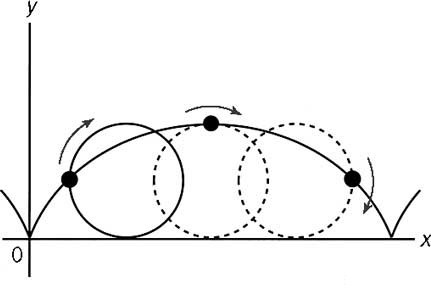
\includegraphics[width=.5\textwidth]{figure/cycloid.jpg}
    %\includegraphics[width=2in]{XeTeX-2.jpg} 
    \caption{the solution is a cycloid (picture from the Internet)}
\end{figure}

\underline{Notes}
\begin{enumerate}
    \item If we have n choice variables, then we need to write EE for each one of them.
    \item In case of higher order derivatives, we can proceed either by
    \begin{itemize}
        \item[a)] introducing new variable, or
        \item[b)] using Euler-Poisson Equation.
    \end{itemize}
\end{enumerate}
\begin{example}
\begin{equation}
    \int_0^T (t y^2 + y y' + {y''}^2) \dd t
\end{equation}
\[
    y(0) = A, ~ y(T) = B, ~ y'(0) = \alpha, ~ y'(T) = \beta
\]
Let: $z = y'$ \imp $z' = y''$

\imp 
$$F = t y^2 + y z + {z'}^2, ~ z(0)=\alpha, ~ z(T) = \beta$$

\imp \begin{equation}
    \begin{cases}
        \int_0^T t y^2 + y z + {z'}^2 \dd t\\[0.5em]
        y(0) = A, ~ y(T) = B, ~z(0)=\alpha, ~ z(T) = \beta
    \end{cases}
\end{equation}
\end{example}

\begin{example} \underline{Continuous Time Dynamic Optimization Model} 
\begin{equation}
    \max \quad \int_0^{\infty} U(C(t))e^{-\delta t} \dd t
\end{equation}        
\begin{equation}
    \text{s.t.} \quad C(t) + B'(t) = \rho(t) B(t) + Y(t)
\end{equation}
where 
\begin{itemize}
    \item [] $C$ = consumption
    \item [] $Y$ = income
    \item [] $B$ = Bonds/Saving
    \item [] $\rho(t)$ = Time-varying interest rate
\end{itemize}
\end{example} 

\underline{General Constained Case}
\begin{equation}
    \max \quad \int_0^{\infty} F(y(t),y'(t),t) \dd t
\end{equation}
\begin{equation}
    \text{s.t.} \quad G(y(t),y'(t),t) = 0, ~\forall t
\end{equation}
The Lagrangian is given by 
$$\mathcal{L} = \int_0^{\infty} F(y(t),y'(t),t) + \lambda(t) G(y(t),y'(t),t) \dd t.$$
\underline{Euler Equation}:
\begin{equation}
    \frac{\pd F}{\pd y(t)} + \lambda(t) \frac{\pd G}{\pd y(t)} - \frac{\dd }{\dd t}\left [ \frac{\pd F}{\pd y'(t)} + \lambda(t) \frac{\pd G}{\pd y'(t)} \right ] = 0
\end{equation}


EE w.r.t. $C(t)$:
\begin{equation}
    U'(C(t))e^{-\delta t} + \lambda(t) = 0
\end{equation}
\begin{equation}
    \Longrightarrow 
    U'(C(t))e^{-\delta t} = - \lambda(t)
\end{equation}
EE w.r.t. $B(t)$:
\begin{equation}
    \lambda(t)(-\rho(t)) - \frac{\dd}{\dd t}[\lambda(t)] = 0
\end{equation}
\begin{equation}
    \Longrightarrow 
    - \lambda(t)\rho(t) = \lambda'(t) 
\end{equation}
(5.26) \imp $$\ln U'(C(t)) - \delta t= \ln (-\lambda(t))$$ \imp $$\frac{1}{U'(C(t))}U''(C(t))C'(t) - \delta = \frac{-\lambda'(t)}{-\lambda(t)} = -\rho(t) $$ 
\imp
\begin{equation}
    - \frac{U''(C(t))}{U'(C(t))}C'(t) = \rho(t) - \delta
\end{equation}
Two equations: (5.21) and (5.29)

Two unknowns: $\{ C_t\}_{t=0}^{\infty}$, $\{ B_t\}_{t=0}^{\infty}$
\begin{equation}
    (5.21) \iff B'(t) - \rho(t)B(t) = Y(t) - C(t) 
\end{equation}
\underline{Recall}
\begin{equation}
    y'(t) + g(t) y(t) = h(t)
\end{equation}
\underline{Forward-looking solution}
\begin{equation}
    y(t) = A e^{-\int_0^t g(v) \dd v } - e^{-\int_0^t g(v) \dd v }\int_t^{\infty} h(s) e^{\int_t^{t+s} g(v) \dd v } \dd s
\end{equation}
 
\underline{Claim:}
$ e^{-\int_0^t \rho(s) \dd s } = \Phi(t)$ is the discount factor when $\rho = \rho(t)$.

If $\rho(t) = \rho$, $\Phi(t) = e^{-\rho t}$.

\begin{equation}
    B(t) = A \underbrace{e^{\int_0^t \rho(v) \dd v }}_{[\Phi(t)]^{-1}} - e^{\int_0^t \rho(v) \dd v } \int_t^{\infty} [ Y(s)-C(s)] e^{-\int_t^{t+s} \rho(v) \dd v } \dd s
\end{equation}

\underline{Assumption}
\begin{itemize}
    \item $\rho(t) = \rho \quad$ \imp $\quad e^{\int_0^t \rho \dd v} = e^{\rho t } = [\Phi(t)]^{-1} $
    \item $Y(t) = Y$ (a constant)
\end{itemize}
\begin{equation}
    B(t) = A [\Phi(t)]^{-1} - [\Phi(t)]^{-1} \int_t^{\infty} \Phi(s) [ Y-C(s)] \dd s
\end{equation}
\begin{equation}
    B(t) = A e^{\rho t} - e^{\rho t} \int_t^{\infty} e^{ - \rho s} [ Y-C(s)] \dd s
\end{equation}
\begin{equation}
    e^{\rho t} \int_t^{\infty} e^{ - \rho s} C(s) \dd s = B(t) + e^{\rho t} \int_t^{\infty} e^{ - \rho s} Y \dd s - A e^{\rho t} 
\end{equation}
If $A >0$, PDV of $C$ shrinks exponentially.

If $A <0$, PDV of $C$ grows exponentially.

\imp $A = 0$

\begin{equation}
    \underbrace{e^{\rho t} \int_t^{\infty} e^{ - \rho s} C(s) \dd s = B(t) + e^{\rho t} \int_t^{\infty} e^{ - \rho s} Y \dd s  }_{\text{life-time budget constraint}}
\end{equation}

\underline{Assumption}
\begin{itemize}
    \item CRRA type utility function $U(C) = \ln C$

    (5.29) \imp ${ \left (- \dfrac{U''}{U'}C \right )} \dfrac{C'}{C} = \rho - \delta,$ 

    where $ -\dfrac{U''}{U'}C $ is the coefficient of relative risk aversion.
\end{itemize}
\imp \begin{equation}
    \frac{C'(t)}{C(t)} = \rho - \delta
\end{equation}
\imp
\begin{equation}
    C(t) = e^{(\rho - \delta)t + a}
\end{equation}
\begin{equation}
    C(s) = e^{(\rho - \delta)(s-t)} C(t)
\end{equation}
(5.37) \imp
\begin{eqnarray}
    e^{\rho t} \int_t^{\infty} e^{ - \rho s} e^{(\rho - \delta)(s-t)} C(t) \dd s &=&  e^{\rho t} \int_t^{\infty} e^{ - \rho s} Y \dd s + B(t)\\
    C(t) e^{\rho t} \int_t^{\infty} e^{ - \rho s} e^{(\rho - \delta)(s-t)}  \dd s &=&  e^{\rho t} Y \int_t^{\infty} e^{ - \rho s} \dd s + B(t)\\
    C(t) e^{\rho t} e^{ \delta t - \rho t} \int_t^{\infty} e^{-\delta s}  \dd s &=&   Y e^{\rho t}\int_t^{\infty} e^{ - \rho s} \dd s + B(t)\\
    C(t) e^{ \delta t} \int_t^{\infty} e^{-\delta s}  \dd s &=&   Y e^{\rho t}\int_t^{\infty} e^{ - \rho s} \dd s + B(t)\\
    C(t)e^{\delta t} (\frac{e^{-\delta t}}{\delta})&=& Ye^{\rho t} (\frac{e^{-\rho t}}{\rho}) + B(t)\\
    \frac{C(t)}{\delta}&=& \frac{Y}{\rho} + B(t)\\
    C(t) &=& \underbrace{\frac{\delta}{\rho}}_{MPC}[Y+\rho B(t)]
\end{eqnarray}

\underline{Backward-looking solution} (applies when $g(t)>0$)

\begin{equation}
    y(t) = A e^{-\int_0^t g(v) \dd v } + \int_0^{\infty} h(t-s) e^{\int_t^{t-s} g(v) \dd v } \dd s
\end{equation}

\section{Discrete time}
\begin{itemize}
    \item [] $P_t = \alpha P_{t-1} + \beta$
    \item [] $P_0 = $ given
    \item [] $P_1 = \alpha P_0 + \beta$
    \item [] $P_2 = \alpha^2 P_0 + \alpha \beta  + \beta$
    \item [] $P_3 = \alpha^3 P_0 + \alpha^2 \beta + \alpha \beta + \beta$
    \item [] $\vdots$
    \item [] $P_t = \alpha^t P_0 + \sum_{i=0}^{t-1} \alpha^i \beta = \alpha^t P_0 + \frac{\beta}{1- \alpha} - \frac{\beta}{1- \alpha} \alpha^t$
    \item [] $P_t = \frac{\beta}{1- \alpha} + (P_0 - \frac{\beta}{1- \alpha})  \alpha^t$
\end{itemize}
If $P_0 = \underbrace{\frac{\beta}{1- \alpha}}_{P^*}$, then $P_t = \frac{\beta}{1- \alpha}$ for all $t$.

\begin{center}
    \texttt{[intert two graphs here for the convergence patterns of $0<\alpha<1$ and $-1<\alpha<0$]} 
\end{center}

$|\alpha| < 1$ -- stable root

$|\alpha| > 1$ -- unstable root

\underline{Lag Operator} (Sargent (1987))
\begin{eqnarray}
    L x_t &=& x_{t-1}\\
    L ( Lx_t) &=& L^2 x_t = x_{t-2}\\
    L^n x_t &=& x_{t-n}\\
    L^{-1}x_t &=& x_{t+1}\\
    L^{-n} x_t &=& x_{t+n}\\
    L^{0} &\equiv& 1
\end{eqnarray}

\underline{Polynomial of Lag Operator}
\begin{equation}
    A(L) = a_0 + a_1 L + a_2 L^2 + ... = \sum_{j=0}^{\infty} a_j L^j
\end{equation}
\begin{equation}
\begin{aligned}
    A(L)x_t &= (a_0 + a_1 L + a_2 L^2 + ...)x_t \\
    &= a_0 x_t + a_1 x_{t-1} + a_2 x_{t-2} + ... \\
    &= \sum_{j=0}^{\infty} a_j x_{t-j}
\end{aligned}
\end{equation}

\underline{Rational Polynomial}
\begin{equation}
    A(L) = \frac{B(L)}{C(L)}
\end{equation}
\begin{example}
    $$AL = \frac{1}{1- \lambda L}$$
    \underline{Claim}: If $|\lambda| <1 $, then \begin{equation}
        \frac{1}{1- \lambda L} = 1 + \lambda L + \lambda^2 L^2 + ... = \sum_{i=0}^{\infty} \lambda^{i} L^{i}
    \end{equation}
    If $|\lambda| >1 $, then \begin{equation}
        \frac{1}{1- \lambda L} = 1 + \frac{\lambda L}{1 - \lambda L} = 1 -  \frac{1}{1 - (\frac{1}{\lambda}) L^{-1}} = 1- (1 + \frac{1}{\lambda} L^{-1} + {\left (\frac{1}{\lambda} \right )}^2 L^{-2} + ...) = - \sum_{i=1}^{\infty} {\left (\frac{1}{\lambda} \right )}^{i} L^{-i}
    \end{equation}
\end{example}





%$$##
\clearpage
\section*{References}
%\beginrefs
%\bibentry{CW87}{\sc D.~Coppersmith} and {\sc S.~Winograd}, 
%``Matrix multiplication via arithmetic progressions,''
%{\it Proceedings of the 19th ACM Symposium on Theory of %Computing},
%1987, pp.~1--6.
%\endrefs

% **** THIS ENDS THE EXAMPLES. DON'T DELETE THE FOLLOWING LINE:

\end{document}












